% !TeX program = pdflatex
%==============================================================================
%  Aula 11 --- KNN e Árvores de Classificação
%  VERSÃO DO ALUNO: texto para leitura autônoma, fora da sala.
%  (O roteiro de sala é "11 KNN e Arvores de Classificacao.tex".)
%==============================================================================
\documentclass[11pt,a4paper]{article}
\usepackage[aluno]{../../recursos/latex/estilo-notas}

\title{}
\date{}

\begin{document}
\cabecalhoaula{11}{KNN e Árvores de Classificação}{AME §8.3--8.6; ISLP §4.7.6 e cap.~8}

%==============================================================================
\section*{O que você vai aprender}
%==============================================================================
Ao final desta aula você deve ser capaz de:
\begin{itemize}[leftmargin=1.4cm]
  \item adaptar o KNN da regressão para classificação e reconhecê-lo como
        classificador \emph{plug-in};
  \item construir uma \textbf{árvore de classificação}, predizendo pela moda da
        folha;
  \item definir \textbf{Gini} e \textbf{entropia} como medidas de impureza e
        explicar por que não se usa a taxa de erro para dividir;
  \item transferir \emph{bagging}, florestas e \emph{boosting} para classificação;
  \item comparar todos os classificadores do curso e escolher segundo a estrutura
        dos dados e o objetivo.
\end{itemize}

\noindent
Esta é a última aula do Bloco~II, e ela fecha um ciclo: praticamente tudo aqui é
uma tradução do Bloco~I, com a média virando \emph{moda} e o EQM virando
\emph{impureza}. Comece pela pergunta:

\begin{center}\itshape
  como uma árvore decide a melhor pergunta a fazer em cada nó,\\
  quando o alvo é uma classe?
\end{center}

\noindent
A resposta ocupa a Seção~\ref{sec:impureza}, e o mais interessante nela é que a
medida \emph{óbvia} --- a taxa de erro --- é justamente a que não funciona.

%==============================================================================
\section{KNN para classificação}
%==============================================================================
Adaptação direta da regressão KNN (Aula~04): para classificar $\x$, olhe seus $k$
vizinhos mais próximos e tome a \textbf{classe mais frequente} (voto da maioria):
\begin{equation}\label{eq:knncls}
  \ghat(\x) = \operatorname{moda}\{Y_i : i\in\mathcal{N}_{\x}\}.
\end{equation}
Equivalentemente, é um classificador \emph{plug-in} (Aula~08): estima-se
\[
  \widehat\Prob(Y=c\mid\x) = \frac{1}{k}\sum_{i\in\mathcal{N}_{\x}}\1{Y_i=c}
\]
(a proporção de vizinhos da classe $c$) e toma-se o $\argmax_c$. Essa estimativa
está, por construção, em $[0,1]$.

\begin{figure}[htbp]
  \centering
  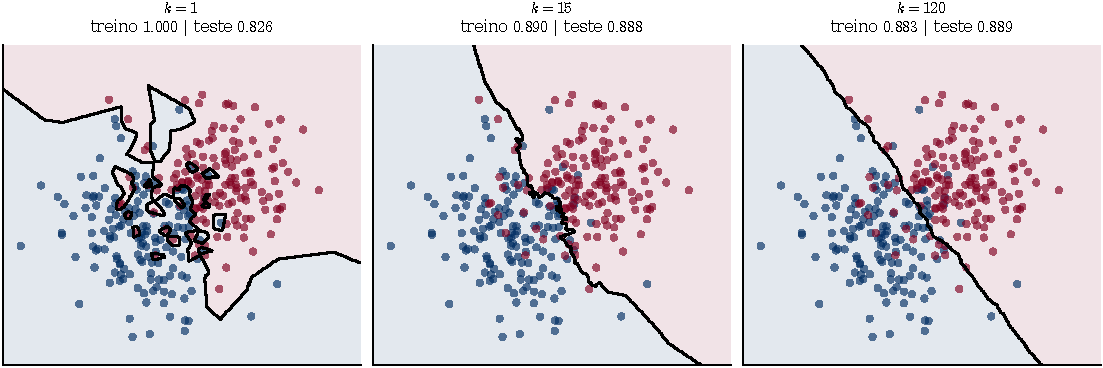
\includegraphics[width=\textwidth]{../../recursos/figuras/11-fronteiras-knn.pdf}
  \caption{Fronteiras de decisão do KNN com $n=300$ pontos de treino, avaliadas em
  $10\,000$ observações novas. Com $k=1$ a fronteira é rendilhada e cria ilhas em
  torno de observações isoladas: a acurácia de treino é \textbf{exatamente $1{,}000$}
  --- cada ponto é seu próprio vizinho mais próximo --- e a de teste é a pior das
  três, $0{,}826$. Com $k=15$ a fronteira suaviza e o teste sobe para $0{,}888$; com
  $k=120$ ela fica quase reta e o teste é praticamente igual, $0{,}889$. Compare com
  a Figura~1 da Aula~04: é o mesmo botão, com a mesma leitura invertida ($k$ pequeno
  $=$ flexível).}
  \label{fig:knncls}
\end{figure}

\begin{ideia}
A acurácia de treino de $1{,}000$ com $k=1$ é o exemplo mais limpo de todo o curso
do que a Aula~01 dizia: o erro de treino é um estimador \emph{otimista} do risco, e
seu otimismo cresce com a flexibilidade. Aqui ele não é só otimista --- é
\emph{perfeito}, e o modelo é o pior dos três. Se alguém lhe mostrar um
classificador com $100\%$ de acerto, a primeira pergunta é ``em qual conjunto?''.
\end{ideia}

\begin{atencao}
Valem os mesmos cuidados da Aula~04: \emph{padronize} as covariáveis (KNN usa
distância) e lembre da \emph{maldição da dimensionalidade} (Aula~05) --- KNN não
seleciona variáveis e degrada com muitas covariáveis irrelevantes. Em binário, use
$k$ \emph{ímpar} para evitar empates.
\end{atencao}

%==============================================================================
\section{Árvores de classificação}
%==============================================================================
São o análogo das árvores de regressão (Aula~06): partição recursiva do espaço de
covariáveis em regiões $R_1,\dots,R_J$. Duas adaptações:

\subsection{Predição: a moda}
Numa folha $R_k$, prediz-se a \textbf{classe majoritária} (em vez da média):
\begin{equation}\label{eq:arvcls}
  \ghat(\x) = \operatorname{moda}\{Y_i : \X_i\in R_k\},\qquad \x\in R_k,
\end{equation}
e $\widehat\Prob(Y=c\mid\x)=\widehat p_{R_k,c}$, a proporção da classe $c$ na folha.
É a substituição que o Teorema de Bayes da Aula~08 previa: em regressão o alvo era
a média condicional, em classificação é a moda condicional.

\subsection{Critério de divisão: impureza}\label{sec:impureza}
O EQM não faz sentido com $Y$ qualitativo. Em cada região $R$, seja
$\widehat p_{R,c}$ a proporção da classe $c$. Buscam-se divisões que tornem as
folhas \textbf{puras} (idealmente, uma só classe por folha). Mede-se a impureza por:
\begin{align}
  \text{Índice de Gini:}\quad & G(R) = \sum_{c\in\mathcal{C}} \widehat p_{R,c}\,(1-\widehat p_{R,c}),
  \label{eq:gini}\\
  \text{Entropia:}\quad & D(R) = -\sum_{c\in\mathcal{C}} \widehat p_{R,c}\,\log \widehat p_{R,c}.
  \label{eq:entropia}
\end{align}
Ambas são \emph{mínimas} (zero) quando a folha é pura (algum $\widehat p_{R,c}=1$) e
\emph{máximas} quando as classes estão equilibradas. A cada passo escolhe-se a
divisão que mais reduz a impureza (ponderada pelo tamanho das folhas).

\begin{figure}[htbp]
  \centering
  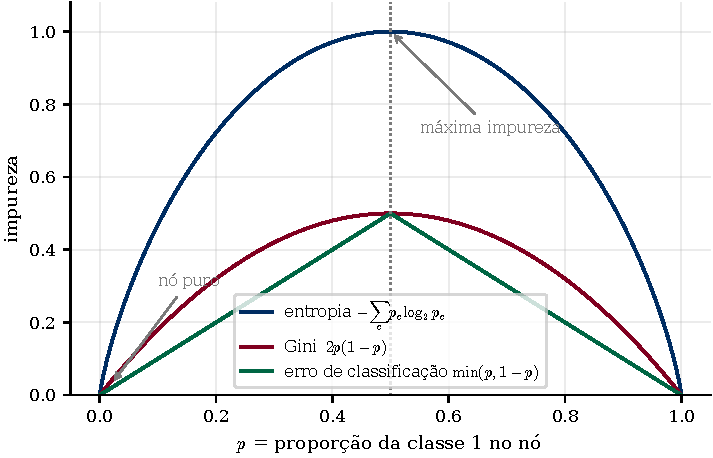
\includegraphics[width=0.62\textwidth]{../../recursos/figuras/11-impureza.pdf}
  \caption{As três medidas num nó binário, em função da proporção $p$ da classe~1.
  Todas zeram nos extremos (nó puro) e são máximas em $p=1/2$. A diferença que
  importa está no \emph{formato}: Gini e entropia são estritamente côncavas e
  suaves, enquanto o erro de classificação é feito de dois segmentos de reta ---
  tem um bico em $p=1/2$ e derivada constante nos dois lados.}
  \label{fig:impureza}
\end{figure}

\begin{ideia}[Por que não usar a taxa de erro para dividir?]
Olhe a curva verde da Figura~\ref{fig:impureza}: ela é \emph{linear} em cada metade.
Isso tem uma consequência devastadora. Suponha um nó com $400$ observações, $\,p=0{,}75$,
e uma divisão que produza duas folhas de $200$ cada, uma com $p=0{,}50$ e outra com
$p=1{,}00$. O erro do pai é $0{,}25$; o erro ponderado dos filhos é
$\tfrac12(0{,}50)+\tfrac12(0{,}00)=0{,}25$. \textbf{Redução zero} --- e no entanto uma
das folhas ficou \emph{pura}, o que é claramente um progresso. Por linearidade, isso
acontece sempre que a classe majoritária não muda. Gini e entropia, sendo
estritamente côncavas, registram qualquer ganho de pureza: no mesmo exemplo o Gini
cai de $0{,}375$ para $0{,}250$. A taxa de erro continua útil na \emph{poda} final,
onde o que interessa é justamente o desempenho de classificação.
\end{ideia}

\begin{exemplo}[Escolha de divisão por Gini]
Para decidir entre dividir por ``Cardiologia'' ou por ``$>100$ leitos'' (predição:
hospital tem tomógrafo), calcula-se o Gini ponderado de cada partição e escolhe-se a
de \emph{menor} valor (maior pureza). No exemplo do [AME], Gini(Leitos)$\approx
0{,}326 <$ Gini(Cardiologia)$\approx 0{,}472$: divide-se por leitos.
\end{exemplo}

\begin{observacao}
Gini e entropia quase sempre escolhem as mesmas divisões --- a diferença numérica
entre as duas curvas da Figura~\ref{fig:impureza} é pequena, e o \emph{argmin} sobre
as divisões candidatas raramente muda. Não vale a pena colocar essa escolha numa
busca por validação cruzada; gaste o orçamento no $\alpha$ de poda ou na
profundidade.
\end{observacao}

\noindent A construção segue as duas etapas da Aula~06: \emph{cresce-se} uma árvore
grande e depois \emph{poda-se} por custo--complexidade ($\alpha$ por CV). As mesmas
vantagens valem: interpretabilidade, categóricas nativas, seleção automática de
variáveis e captura de interações --- e a mesma desvantagem, os cortes
perpendiculares aos eixos.

%==============================================================================
\section{\emph{Ensembles} para classificação}
%==============================================================================
Toda a Aula~06 se transfere; as árvores individuais agora classificam:
\begin{description}[leftmargin=2.6cm,style=nextline]
  \item[Bagging / Florestas] treina $B$ árvores em amostras bootstrap e agrega por
        \textbf{voto da maioria} (ou média das probabilidades --- em geral melhor,
        porque preserva alguma informação sobre a confiança). Florestas
        descorrelacionam sorteando $m$ variáveis por nó; regra empírica em
        classificação: $m\approx\sqrt{d}$, mais agressiva que o $d/3$ da regressão.
        Robustas a $B$; OOB e importância de variáveis ``de graça''.
  \item[Boosting] ajuste sequencial. A variante clássica para classificação é o
        \textbf{AdaBoost}: a cada rodada, reponderam-se as observações dando mais
        peso às mal classificadas, e o classificador final é um voto ponderado dos
        aprendizes fracos. Como em regressão, $B$ grande pode superajustar (use
        \emph{early stopping}); XGBoost é a implementação de referência.
\end{description}

\begin{observacao}
Vale registrar a ponte teórica: o AdaBoost, apesar de ter sido inventado por outro
caminho, equivale a fazer \emph{boosting} com a \textbf{perda exponencial}
$e^{-y\,g(\x)}$ --- mais uma perda de margem, no mesmo eixo horizontal da
Figura~4 da Aula~10. Vista assim, ela é ainda mais agressiva que a \emph{hinge} com
os pontos mal classificados, o que explica a sensibilidade conhecida do AdaBoost a
rótulos errados.
\end{observacao}

%==============================================================================
\section{Comparando os classificadores do curso}
%==============================================================================
\begin{center}\small
\renewcommand{\arraystretch}{1.3}
\begin{tabular}{@{}lp{3.5cm}p{3.2cm}p{3.6cm}@{}}
\toprule
\textbf{Método} & \textbf{Fronteira} & \textbf{Interpretab.} & \textbf{Observações} \\
\midrule
Logística & linear (no \emph{log-odds}) & alta (coefs.) & dá probabilidades; robusta \\
LDA / QDA & linear / quadrática & média & ótimos sob gaussianidade \\
Bayes ingênuo & depende & média & forte com texto; descalibra se há correlação \\
KNN & muito flexível, local & baixa & sensível a escala e dimensão \\
Árvore & ``escada'' (eixos) & \textbf{altíssima} & instável sozinha \\
Florestas / Boosting & muito flexível & baixa & topo de desempenho em dados tabulares \\
SVM (kernel) & linear ou não linear & baixa & ótima com classes separadas \\
\bottomrule
\end{tabular}
\end{center}

\begin{ideia}
Não há método universalmente melhor (Aula~05: ``não existe almoço grátis''). A
escolha depende da \emph{estrutura} dos dados e do \emph{objetivo}. Quatro perguntas
que resolvem a maioria dos casos:
\begin{enumerate}[leftmargin=1.6cm,nosep]
  \item \textbf{Preciso de probabilidades calibradas?} Se sim, logística; se não,
        qualquer um (Aula~09).
  \item \textbf{Preciso explicar a decisão a alguém?} Se sim, árvore ou logística.
  \item \textbf{Há muitas covariáveis irrelevantes?} Então evite KNN e SVM-RBF, que
        somam todas as coordenadas na distância; prefira Lasso, florestas ou
        \emph{boosting} (Aula~05).
  \item \textbf{Os dados são tabulares e o objetivo é acertar?} Comece por
        \emph{boosting} de árvores --- é o que costuma ganhar --- e use os outros como
        referência.
\end{enumerate}
E, em qualquer caso, compare os candidatos por validação cruzada com a métrica
adequada ao problema.
\end{ideia}

%==============================================================================
\section{Prática em Python}
%==============================================================================
\begin{lstlisting}
from sklearn.neighbors import KNeighborsClassifier
from sklearn.tree import DecisionTreeClassifier, plot_tree
from sklearn.ensemble import RandomForestClassifier, GradientBoostingClassifier

# KNN: k impar, padronizado dentro do pipeline (Aula 07)
knn = make_pipeline(StandardScaler(), KNeighborsClassifier(n_neighbors=11))

# Arvore: criterion "gini" (padrao) ou "entropy" -- na pratica, tanto faz
arv = DecisionTreeClassifier(criterion="gini", ccp_alpha=0.01).fit(X_tr, y_tr)
plot_tree(arv, feature_names=nomes, class_names=classes, filled=True)

# Floresta: m = sqrt(d) e o padrao em classificacao
rf = RandomForestClassifier(n_estimators=500, max_features="sqrt",
                            oob_score=True, random_state=0).fit(X_tr, y_tr)
\end{lstlisting}
Repare que \texttt{max\_features="sqrt"} já é o padrão do
\texttt{RandomForestClassifier}, enquanto no \texttt{RandomForestRegressor} o padrão
é usar todas as variáveis --- isto é, \emph{bagging}, não floresta. Se você quer uma
floresta em regressão, precisa dizer.

Os notebooks \texttt{Aula prática 11}, \texttt{Comparação entre classificadores
paramétricos} e
\texttt{Exemplo - KNN e árvores em dados artificiais} desenham as fronteiras de
decisão de todos esses métodos lado a lado, nos mesmos dados. É o melhor jeito de
fixar a intuição de ``flexível $\times$ rígido'' que percorreu o curso inteiro ---
vale rodar os dois.

%==============================================================================
\section*{Resumo}
%==============================================================================
\begin{itemize}[leftmargin=1.4cm]
  \item \textbf{KNN} \eqref{eq:knncls}: voto da maioria entre os $k$ vizinhos; é
        \emph{plug-in} com $\widehat\Prob$ igual à proporção local. Com $k=1$ o
        treino dá $100\%$ e o teste dá o pior resultado (Fig.~\ref{fig:knncls}).
  \item \textbf{Árvore de classificação} \eqref{eq:arvcls}: prediz a moda da folha;
        divide minimizando \textbf{Gini} \eqref{eq:gini} ou \textbf{entropia}
        \eqref{eq:entropia}.
  \item A \emph{taxa de erro} não serve para dividir porque é linear por partes e
        registra redução zero em divisões que aumentam a pureza
        (Fig.~\ref{fig:impureza}); serve para podar.
  \item \emph{Ensembles} transferem-se inteiros: florestas com $m\approx\sqrt d$,
        AdaBoost como \emph{boosting} com perda exponencial.
  \item Não há método universalmente melhor: escolha pela estrutura dos dados e
        pelo objetivo, e compare por validação cruzada com a métrica certa
        (Aula~09).
\end{itemize}

\paragraph{Leitura recomendada.} [AME] §8.3 (árvores de classificação, com o
exemplo do tomógrafo reproduzido aqui), §8.4--8.5 (\emph{bagging}, florestas e
\emph{boosting} em classificação) e §8.6 (KNN). [ISLP] §4.7.6 (KNN) e Capítulo~8
--- §8.1.2 trata especificamente das árvores de classificação e dos critérios de
impureza, com a versão deles da nossa Figura~\ref{fig:impureza}.

\paragraph{Para praticar.} \texttt{recursos/listas/Lista de exercícios 08.pdf}.

\end{document}
